Объектом исследования является множество сайтов характеризуемых некоторым набором признаков.
Рассмотрим одноклассовую классификацию объектов генеральной совокупности $\Omega$.
Пусть каждый объект $\omega \in{\Omega}$  представлен точкой в линейном пространстве признаков
$\mathbf{x}(\omega)=\cbr{x^1(\omega),\ldots, x^n(\omega)} \in {\mathbb{R}^n}$,
а его скрытая фактическая принадлежность или не принадлежность к классу
определяется значением $y(\omega)\in{\{0,1\}}$. Будем строить сферический пороговый классификатор
$z(\mathbf{x},\mathbf{a},R)=\left\|\mathbf{x}-\mathbf{a}\right\|-R$. Множество $\Omega^*$ объектов 
$x_j, j=1 \ldots N$ на которых известна скрытая характеристика $y_j$, назовем обучающей совокупностью. 
В обучающей совокупности будут только объекты класса, то есть $y_j=1$ для всех $j=1\ldots N$.

\begin{figure}[H]
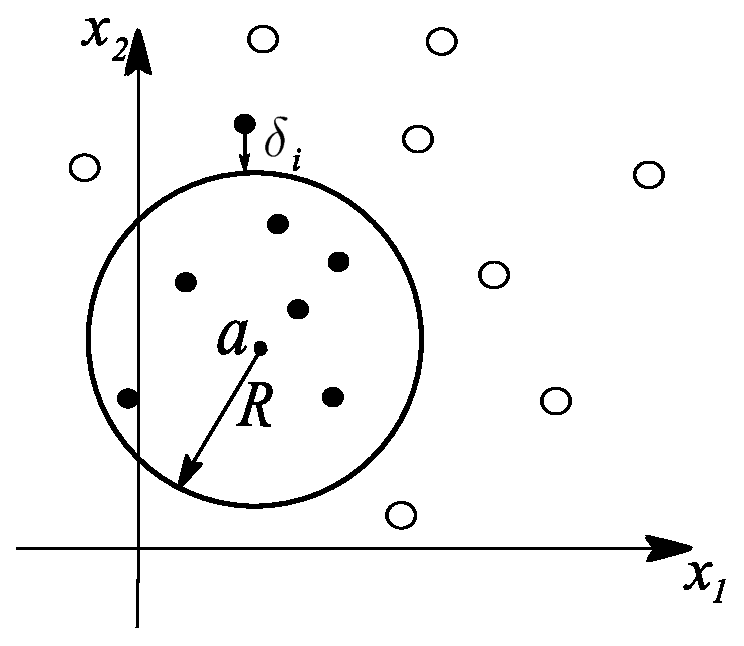
\includegraphics[width=150px, height=130px]{fig1.eps}
\end{figure}

Будем придерживаться вероятностной модели распределения объектов генеральной совокупности. 
Параметрическое семейство условных плотностей распределения в признаковом пространстве имеет вид 
\begin{equation}
\label{prob1}
	\varphi \cbr{ {\mathbf x | y,\mathbf{a},R;c} } =
	\begcas{
		&\text{const},		\qquad\,					z(\mathbf{x},\mathbf{a},R) \geq 0, \\
		&e^{-c z(\mathbf{x},\mathbf{a},R)},\;	z(\mathbf{x},\mathbf{a},R) \leq 0.
	} 
\vspace{-5pt}
\end{equation}

\begin{figure}[H]
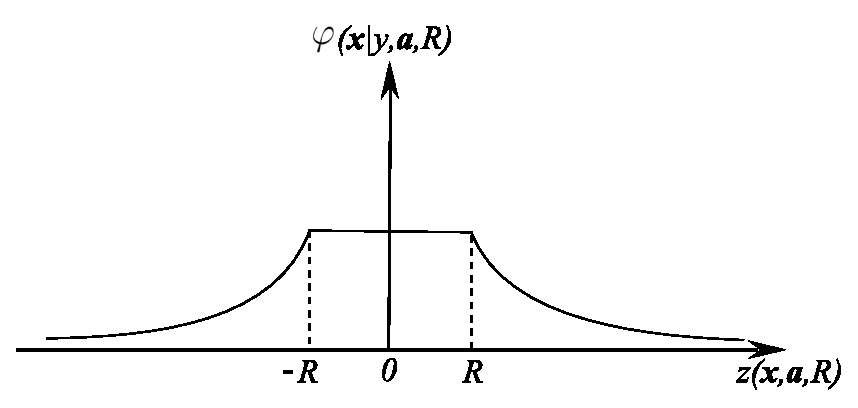
\includegraphics[width=200px, height=100px]{fig2.eps}
\caption{Значение плотности распределения вдоль радиуса}
\end{figure}

Совместную плотность распределения случайной обучающей совокупности будем понимать как плотность 
распределения выборки независимых реализаций
$$\Phi(\mathbf{X}|Y,\mathbf{a},R)=\prod \limits_{j=1}^N \varphi(\mathbf{x}_j|y_j,\mathbf{a},R),$$ 
где $\mathbf{X}= \fbr{\mathbf{x}}_{j=1}^N$, а $Y = \fbr{y_j}_{j=1}^N$.
Пусть, далее, выбрана априорная плотность совместного распределения вероятностей $\Psi(\mathbf{a},R)$ 
для параметров распределения $\varphi \cbr{\mathbf x | y,\mathbf{a},R;c}$. Тогда апостериорная
 плотность распределения параметров $\mathbf{a}$ и $R$ относительно обучающей совокупности определяется 
формулой Байеса
$$p(\mathbf{a},R|\mathbf{X},Y)=\frac{\Psi(\mathbf{a},R) \Phi(\mathbf{X}|Y,\mathbf{a},R)}
{\int {\Psi(\mathbf{a}',R') \Phi(\mathbf{X}|Y,\mathbf{a}',R')d\mathbf{a}'dR'}}.$$
Поскольку знаменатель не зависит от целевых переменных, о достаточно рассматривать только числитель
$$p(\mathbf{a},R|\mathbf{X},Y) \propto \Psi(\mathbf{a},R) \Phi(\mathbf{X}|Y,\mathbf{a},R) = 
\Psi(\mathbf{a},R) \prod \limits_{j=1}^N \varphi(\mathbf{x}_j|y_j,\mathbf{a},R).$$
Из принципа максимума плотности апостериорного распределения в пространстве параметров модели генеральной
 совокупности получим байесовское правило обучения
$$\cbr{\hat{\mathbf{a}},\hat{R}|\mathbf{X},Y}
	= \arg\underset{\mathbf{a},R}{\max}\;\; p(\mathbf{a},R|\mathbf{X},Y) 
	= \arg\underset{\mathbf{a},R}{\max}\;\; {\log}\Psi(\mathbf{a},R) + \sum\limits_{j=1}^N{\log}\varphi(\mathbf{x}_j|y_j,\mathbf{a},R) $$


